\documentclass{beamer}
\usetheme{Madrid}
\usecolortheme{default}

\usepackage{listings}
\usepackage{xcolor}
\usepackage{tikz}
\usetikzlibrary{shapes,arrows,positioning}

\lstset{
    language=C++,
    basicstyle=\tiny\ttfamily,
    keywordstyle=\color{blue}\bfseries,
    commentstyle=\color{green!60!black},
    stringstyle=\color{red},
    showstringspaces=false,
    breaklines=true,
    frame=single,
    backgroundcolor=\color{gray!10},
    morekeywords={pragma,omp,parallel,single,task,taskwait,critical,atomic,shared,firstprivate}
}

\title{OpenMP Parallelization in ConTree}
\subtitle{Optimal Decision Tree Solver - CS406 Project}
\author[]{Borhan Javadian \and Emre Ute \and Harun Yilmaz \and \\ Deniz Kaan Yilmaz \and Tolga Toker \and Yusuf Demirci}
\institute{Group 2}
\date{\today}

\begin{document}

\frame{\titlepage}

%===============================================================================
\begin{frame}{Presentation Outline}
\tableofcontents
\end{frame}

%===============================================================================
\section{Problem Overview}

\begin{frame}{What is ConTree?}
\begin{block}{Optimal Decision Tree Solver}
ConTree finds \textbf{provably optimal} decision trees using branch-and-bound search.
\end{block}

\vspace{0.5em}
\textbf{Computational Challenge:}
\begin{itemize}
    \item Exhaustive search over all features and split points
    \item Recursive tree construction (exponential complexity)
    \item Depth-2 trees solved by specialized algorithm
\end{itemize}

\vspace{0.5em}
\begin{alertblock}{Goal}
Parallelize the search to reduce computation time while maintaining correctness.
\end{alertblock}
\end{frame}

%===============================================================================
\section{Parallelization Architecture}

\begin{frame}{Three-Level Parallel Architecture}
\begin{center}
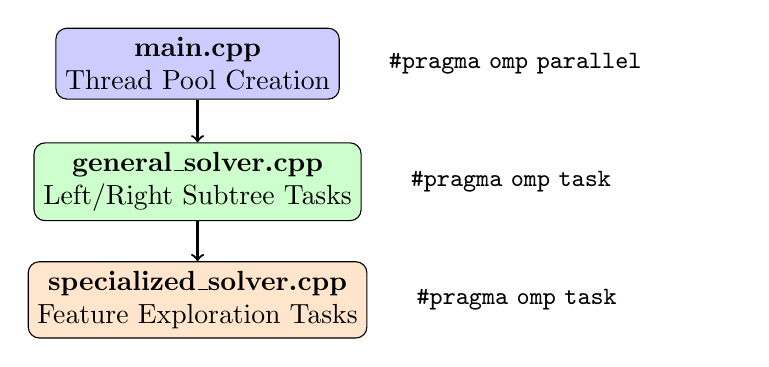
\begin{tikzpicture}[
    box/.style={rectangle, draw, rounded corners, minimum width=3cm, minimum height=0.8cm, align=center},
    arrow/.style={->, thick}
]
    \node[box, fill=blue!20] (main) at (0,3) {\textbf{main.cpp}\\Thread Pool Creation};
    \node[box, fill=green!20] (general) at (0,1.5) {\textbf{general\_solver.cpp}\\Left/Right Subtree Tasks};
    \node[box, fill=orange!20] (special) at (0,0) {\textbf{specialized\_solver.cpp}\\Feature Exploration Tasks};
    
    \draw[arrow] (main) -- (general);
    \draw[arrow] (general) -- (special);
    
    \node[right=0.5cm of main, text width=4cm, font=\small] {\texttt{\#pragma omp parallel}};
    \node[right=0.5cm of general, text width=4cm, font=\small] {\texttt{\#pragma omp task}};
    \node[right=0.5cm of special, text width=4cm, font=\small] {\texttt{\#pragma omp task}};
\end{tikzpicture}
\end{center}

\begin{block}{Key Design: Tasks, Not Nested Regions}
All parallelism uses \textbf{OpenMP tasks} within a single parallel region.\\
This avoids the overhead of creating nested thread teams.
\end{block}
\end{frame}

%===============================================================================
\section{Level 1: main.cpp - Thread Pool}

\begin{frame}[fragile]{main.cpp: Creating the Thread Pool}
\begin{lstlisting}
// Start parallel region at top level for task-based parallelism
#pragma omp parallel
{
    #pragma omp single
    {
        GeneralSolver::create_optimal_decision_tree(
            dataview, config, optimal_decision_tree, INT_MAX);
    }
}
\end{lstlisting}

\vspace{0.5em}
\textbf{Step-by-step:}
\begin{enumerate}
    \item \texttt{\#pragma omp parallel} creates a \textbf{team of threads} (default: all CPU cores)
    \item \texttt{\#pragma omp single} ensures only \textbf{one thread} starts the computation
    \item Other threads \textbf{wait in the pool}, ready to execute tasks
    \item When tasks are created later, idle threads pick them up
\end{enumerate}
\end{frame}

\begin{frame}{Why parallel + single?}
\begin{columns}
\column{0.5\textwidth}
\textbf{Without parallel region:}
\begin{itemize}
    \item Tasks have no threads to run on
    \item Everything executes sequentially
    \item \texttt{\#pragma omp task} is ignored
\end{itemize}

\column{0.5\textwidth}
\textbf{With parallel + single:}
\begin{itemize}
    \item Thread pool is ready
    \item One thread does initial work
    \item Tasks distributed to idle threads
\end{itemize}
\end{columns}

\vspace{1em}
\begin{alertblock}{Critical Insight}
The parallel region is created \textbf{once at the top level}.\\
All nested functions use \textbf{tasks only} - no new parallel regions!
\end{alertblock}
\end{frame}

%===============================================================================
\section{Level 2: general\_solver.cpp - Subtree \& Feature Parallelism}

\begin{frame}[fragile]{General Solver: Feature Parallelization}
The general solver explores all features as potential root splits:
\begin{lstlisting}
// Parallel feature exploration 
for (int feature_nr = 0; feature_nr < dataview.get_feature_number(); feature_nr++) {
    int feature_index = dataview.gini_values[feature_nr].second;
    
    #pragma omp task firstprivate(feature_index) \
                     shared(current_optimal_decision_tree, dataview, ...)
    {
        int current_upper_bound;
        #pragma omp atomic read
        current_upper_bound = current_optimal_decision_tree->misclassification_score;
        
        if (current_upper_bound > 0 && solution_configuration.stopwatch.IsWithinTimeLimit()) {
            create_optimal_decision_tree(dataview, ..., feature_index, ...);
        }
    }
}
#pragma omp taskwait
\end{lstlisting}

\textbf{Key insight:} Each feature can be explored \textbf{independently} as a task!
\end{frame}

\begin{frame}[fragile]{General Solver: Subtree Independence}
For each candidate split point, we need to evaluate:
\begin{itemize}
    \item \textbf{Left subtree}: Optimal tree for data points $\leq$ threshold
    \item \textbf{Right subtree}: Optimal tree for data points $>$ threshold
\end{itemize}

\vspace{0.5em}
\textbf{Key observation:} Left and right are \textbf{completely independent}!

\begin{lstlisting}
Dataview left_dataview = ...;   // Separate copy
Dataview right_dataview = ...;  // Separate copy

std::shared_ptr<Tree> left_optimal_dt = ...;  // Own output
std::shared_ptr<Tree> right_optimal_dt = ...; // Own output

// These two calls don't share any state!
GeneralSolver::create_optimal_decision_tree(left_dataview, ..., left_optimal_dt);
GeneralSolver::create_optimal_decision_tree(right_dataview, ..., right_optimal_dt);
\end{lstlisting}
\end{frame}

\begin{frame}[fragile]{General Solver: Parallel Subtree Tasks}
\begin{lstlisting}
// Task granularity cutoff: avoid overhead for small problems
const int min_dataset_size_for_parallel = 1000;
const int min_depth_for_parallel = 3;
const bool should_parallelize = 
    (solution_configuration.max_depth >= min_depth_for_parallel) && 
    (dataview.get_dataset_size() >= min_dataset_size_for_parallel);

if (should_parallelize) {
    // Create task for LEFT subtree
    #pragma omp task shared(left_dataview, left_optimal_dt)
    {
        GeneralSolver::create_optimal_decision_tree(
            left_dataview, left_solution_configuration, left_optimal_dt, ...);
    }
    
    // Create task for RIGHT subtree
    #pragma omp task shared(right_dataview, right_optimal_dt)
    {
        GeneralSolver::create_optimal_decision_tree(
            right_dataview, right_solution_configuration, right_optimal_dt, ...);
    }
    
    #pragma omp taskwait  // Wait for BOTH to complete before using results
}
\end{lstlisting}
\end{frame}

\begin{frame}{Granularity Cutoff: Why It Matters}
\begin{columns}
\column{0.5\textwidth}
\textbf{Problem: Task Overhead}
\begin{itemize}
    \item Creating a task has cost
    \item Scheduling adds latency
    \item Small tasks: overhead $>$ benefit
\end{itemize}

\column{0.5\textwidth}
\textbf{Solution: Cutoff Thresholds}
\begin{itemize}
    \item Depth $\geq$ 3 (enough work)
    \item Dataset $\geq$ 1000 points
    \item Below threshold: run sequentially
\end{itemize}
\end{columns}

\vspace{1em}
\begin{exampleblock}{Example}
\begin{tabular}{|l|c|c|}
\hline
\textbf{Situation} & \textbf{Depth} & \textbf{Parallelize?} \\
\hline
Root problem & 5 & Yes (if size $\geq$ 1000) \\
\hline
Near leaves & 1 & No (too shallow) \\
\hline
Small subset & any & No (dataset too small) \\
\hline
\end{tabular}
\end{exampleblock}
\end{frame}

%===============================================================================
\section{Level 3: specialized\_solver.cpp - Feature Parallelism}

\begin{frame}{Specialized Solver: Depth-2 Optimization}
For depth-2 trees, we use an optimized algorithm:
\begin{itemize}
    \item No recursion needed
    \item Direct computation of depth-1 subtrees
    \item Explores all \textbf{features} as potential root splits
\end{itemize}

\vspace{0.5em}
\textbf{Parallelization opportunity:}
\begin{itemize}
    \item Each feature can be explored \textbf{independently}
    \item But they all update the \textbf{same best tree} (shared state!)
\end{itemize}

\begin{alertblock}{Challenge}
Unlike general solver, we have \textbf{shared mutable state} - the best tree found so far.
This requires \textbf{synchronization}.
\end{alertblock}
\end{frame}

\begin{frame}[fragile]{Specialized Solver: Feature Exploration Tasks}
\begin{lstlisting}
void SpecializedSolver::create_optimal_decision_tree(
    const Dataview& dataview, const Configuration& solution_configuration,
    std::shared_ptr<Tree>& current_optimal_decision_tree, int upper_bound) 
{
    const int feature_count = dataview.get_feature_number();
    
    // Create a task for EACH feature
    for (int feature_index = 0; feature_index < feature_count; feature_index++) {
        #pragma omp task firstprivate(feature_index) \
                         shared(current_optimal_decision_tree, dataview, ...)
        {
            // Each task explores one feature as root split
            int current_score;
            #pragma omp critical(specialized_tree_access)
            {
                current_score = current_optimal_decision_tree->misclassification_score;
            }
            
            if (current_score > solution_configuration.max_gap) {
                create_optimal_decision_tree(..., feature_index, 
                    current_optimal_decision_tree, ...);
            }
        }
    }
    #pragma omp taskwait  // Wait for all features to be explored
}
\end{lstlisting}
\end{frame}

\begin{frame}[fragile]{Critical Sections: Protecting Shared State}
\textbf{Problem:} Multiple tasks read/write \texttt{current\_optimal\_decision\_tree}

\vspace{0.5em}
\textbf{Solution:} Use \texttt{critical} sections with a \textbf{named lock}

\begin{lstlisting}
// Reading current best score (before doing work)
#pragma omp critical(specialized_tree_access)
{
    current_score = current_optimal_decision_tree->misclassification_score;
}

// Updating the tree (after finding potentially better solution)
#pragma omp critical(specialized_tree_access)
{
    // Double-check pattern: re-verify inside lock
    if (current_best_score < current_optimal_decision_tree->misclassification_score) {
        current_optimal_decision_tree->misclassification_score = current_best_score;
        current_optimal_decision_tree->update_split(feature_index, threshold, ...);
    }
    current_misclassification = current_optimal_decision_tree->misclassification_score;
}
\end{lstlisting}
\end{frame}

\begin{frame}{Why Named Critical Sections?}
\begin{block}{Syntax: \texttt{\#pragma omp critical(name)}}
All critical sections with the \textbf{same name} use the \textbf{same lock}.
\end{block}

\vspace{0.5em}
We use \texttt{specialized\_tree\_access} in three places:
\begin{enumerate}
    \item \textbf{Line 50-53}: Read score before starting feature exploration
    \item \textbf{Line 254-257}: Read score for pruning decisions
    \item \textbf{Line 287-296}: Write updated tree (with double-check)
\end{enumerate}

\vspace{0.5em}
\begin{alertblock}{Double-Check Pattern}
We re-check the condition \textbf{inside} the lock because another thread may have updated the tree between our computation and our attempt to write.
\end{alertblock}
\end{frame}

\begin{frame}[fragile]{Atomic Operations for Statistics}
For simple counters, use \texttt{atomic} instead of \texttt{critical}:

\begin{lstlisting}
#pragma omp atomic
statistics::total_number_of_specialized_solver_calls += 1;
\end{lstlisting}

\vspace{1em}
\begin{columns}
\column{0.5\textwidth}
\textbf{atomic}
\begin{itemize}
    \item Single memory operation
    \item Hardware-level guarantee
    \item Very low overhead
    \item Limited to simple operations
\end{itemize}

\column{0.5\textwidth}
\textbf{critical}
\begin{itemize}
    \item Arbitrary code block
    \item Software lock
    \item Higher overhead
    \item More flexible
\end{itemize}
\end{columns}
\end{frame}

%===============================================================================
\section{Avoiding Nested Parallelism}

\begin{frame}{The Nested Parallelism Trap}
\begin{alertblock}{What We Tried (and Failed)}
Initially, we added \texttt{\#pragma omp parallel} inside specialized\_solver:
\begin{itemize}
    \item Created a \textbf{new team of threads} for each call
    \item When called from general\_solver tasks: \textbf{nested teams}!
    \item Result: 4x \textbf{slower} than sequential (25s vs 6.7s)
\end{itemize}
\end{alertblock}

\vspace{0.5em}
\begin{block}{Why It's Slow}
\begin{itemize}
    \item Thread creation is expensive
    \item Nested teams compete for same CPU cores
    \item Synchronization overhead multiplies
    \item Cache thrashing between thread teams
\end{itemize}
\end{block}
\end{frame}

\begin{frame}{The Solution: Tasks Only}
\begin{center}
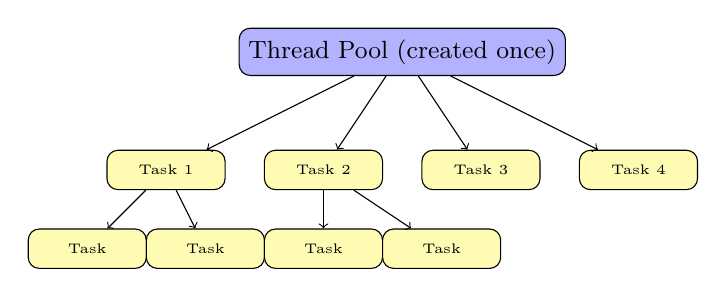
\begin{tikzpicture}[
    box/.style={rectangle, draw, rounded corners, minimum width=2.5cm, minimum height=0.6cm, align=center, font=\small},
    task/.style={rectangle, draw, rounded corners, minimum width=1.5cm, minimum height=0.5cm, align=center, font=\tiny, fill=yellow!30}
]
    \node[box, fill=blue!30] (pool) at (0,2.5) {Thread Pool (created once)};
    
    \node[task] (t1) at (-3,1) {Task 1};
    \node[task] (t2) at (-1,1) {Task 2};
    \node[task] (t3) at (1,1) {Task 3};
    \node[task] (t4) at (3,1) {Task 4};
    
    \node[task] (t1a) at (-4,0) {Task};
    \node[task] (t1b) at (-2.5,0) {Task};
    \node[task] (t2a) at (-1,0) {Task};
    \node[task] (t2b) at (0.5,0) {Task};
    
    \draw[->] (pool) -- (t1);
    \draw[->] (pool) -- (t2);
    \draw[->] (pool) -- (t3);
    \draw[->] (pool) -- (t4);
    \draw[->] (t1) -- (t1a);
    \draw[->] (t1) -- (t1b);
    \draw[->] (t2) -- (t2a);
    \draw[->] (t2) -- (t2b);
\end{tikzpicture}
\end{center}

\textbf{All tasks share the same thread pool:}
\begin{itemize}
    \item No thread creation overhead after initial pool
    \item Tasks from any level can run on any thread
    \item Natural work-stealing and load balancing
\end{itemize}
\end{frame}

%===============================================================================
\section{Performance Results}

\begin{frame}[fragile]{Running the Solver: run\_smart.sh}
We use a smart wrapper script to configure OpenMP settings:

\begin{lstlisting}[language=bash]
#!/bin/bash
# Automatically selects optimal OMP settings based on depth

export OMP_DYNAMIC=false

if [ "$DEPTH" -le 3 ]; then
    export OMP_NUM_THREADS=60
    export OMP_PLACES=cores
    export OMP_PROC_BIND=spread
    export OMP_WAIT_POLICY=active
else
    export OMP_NUM_THREADS=60  # or 30 for specific datasets, specifically raisin
fi

# Use NUMA interleaved memory allocation
exec numactl --interleave=all "$@"
\end{lstlisting}

\textbf{Usage:} \texttt{./run\_smart.sh ./ConTree -file data.txt -max-depth 3}
\end{frame}

\begin{frame}{Benchmark Results: Overview}
\textbf{Configuration:} 60 threads (30 for raisin), SPREAD binding, 10 runs averaged

\vspace{0.3em}
\begin{table}
\centering
\small
\begin{tabular}{|l|c|c|c|c|}
\hline
\textbf{Dataset} & \textbf{Depth} & \textbf{Time (s)} & \textbf{Score} & \textbf{Accuracy} \\
\hline
avila.txt & 3 & 2.0046 & 8664 & 58.5\% \\
\hline
bean.txt & 3 & 2.3136 & 1748 & 87.2\% \\
\hline
raisin.txt & 4 & 6.0740 & 74 & 91.8\% \\
\hline
segment.txt & 4 & 6.9763 & 101 & 95.6\% \\
\hline
\end{tabular}
\end{table}

\vspace{0.3em}
\begin{block}{Key Observations}
\begin{itemize}
    \item Depth-4 problems take 2.5-3x longer than depth-3
    \item Higher accuracy correlates with fewer misclassifications
    \item Thread count tuned per dataset (raisin benefits from 30 threads)
\end{itemize}
\end{block}
\end{frame}

\begin{frame}{Benchmark Results: Execution Time}
\begin{center}
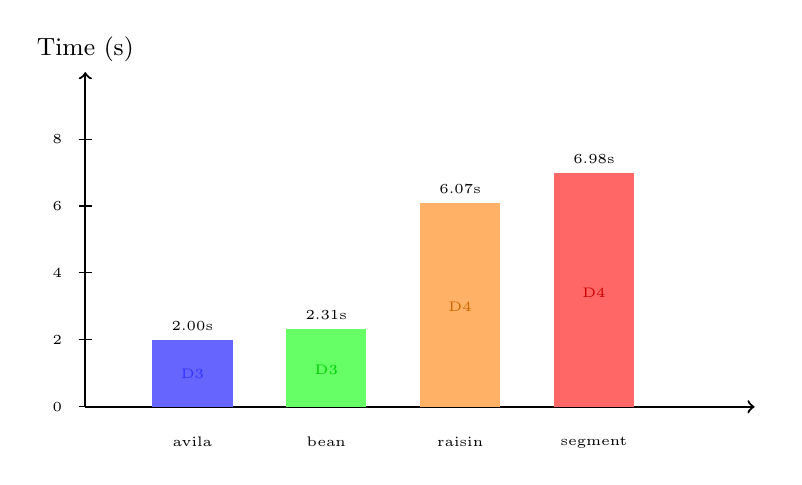
\begin{tikzpicture}[scale=0.85]
    % Bar chart for execution time
    \draw[thick,->] (0,0) -- (10,0) node[right] {};
    \draw[thick,->] (0,0) -- (0,5) node[above] {\small Time (s)};
    
    % Y-axis labels
    \foreach \y/\label in {0/0, 1/2, 2/4, 3/6, 4/8} {
        \draw (-0.1,\y) -- (0.1,\y);
        \node[left] at (-0.2,\y) {\tiny \label};
    }
    
    % Bars (scaled: 1 unit = 2 seconds)
    \fill[blue!60] (1,0) rectangle (2.2,1.00);
    \fill[green!60] (3,0) rectangle (4.2,1.16);
    \fill[orange!60] (5,0) rectangle (6.2,3.04);
    \fill[red!60] (7,0) rectangle (8.2,3.49);
    
    % Labels
    \node[below, font=\tiny] at (1.6,-0.3) {avila};
    \node[below, font=\tiny] at (3.6,-0.3) {bean};
    \node[below, font=\tiny] at (5.6,-0.3) {raisin};
    \node[below, font=\tiny] at (7.6,-0.3) {segment};
    
    % Values on top
    \node[above, font=\tiny] at (1.6,1.00) {2.00s};
    \node[above, font=\tiny] at (3.6,1.16) {2.31s};
    \node[above, font=\tiny] at (5.6,3.04) {6.07s};
    \node[above, font=\tiny] at (7.6,3.49) {6.98s};
    
    % Depth annotations
    \node[font=\tiny, blue!80] at (1.6,0.5) {D3};
    \node[font=\tiny, green!80!black] at (3.6,0.55) {D3};
    \node[font=\tiny, orange!80!black] at (5.6,1.5) {D4};
    \node[font=\tiny, red!80!black] at (7.6,1.7) {D4};
\end{tikzpicture}
\end{center}

\vspace{0.3em}
\textbf{Insight:} Depth-4 problems show exponential growth in search space, resulting in 2.5-3x longer execution times compared to depth-3 problems.
\end{frame}

\begin{frame}{Benchmark Results: Accuracy}
\begin{center}
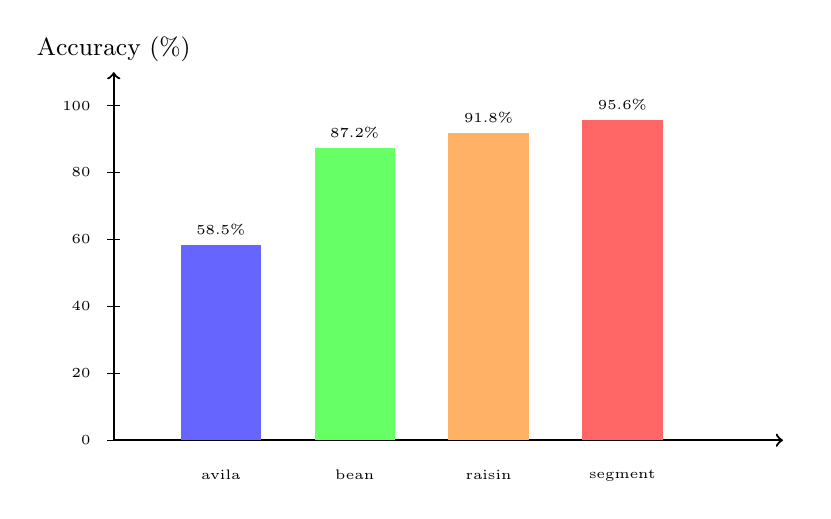
\begin{tikzpicture}[scale=0.85]
    % Bar chart for accuracy
    \draw[thick,->] (0,0) -- (10,0) node[right] {};
    \draw[thick,->] (0,0) -- (0,5.5) node[above] {\small Accuracy (\%)};
    
    % Y-axis labels
    \foreach \y/\label in {0/0, 1/20, 2/40, 3/60, 4/80, 5/100} {
        \draw (-0.1,\y) -- (0.1,\y);
        \node[left] at (-0.2,\y) {\tiny \label};
    }
    
    % Bars (scaled: 100% = 5 units)
    \fill[blue!60] (1,0) rectangle (2.2,2.92);
    \fill[green!60] (3,0) rectangle (4.2,4.36);
    \fill[orange!60] (5,0) rectangle (6.2,4.59);
    \fill[red!60] (7,0) rectangle (8.2,4.78);
    
    % Labels
    \node[below, font=\tiny] at (1.6,-0.3) {avila};
    \node[below, font=\tiny] at (3.6,-0.3) {bean};
    \node[below, font=\tiny] at (5.6,-0.3) {raisin};
    \node[below, font=\tiny] at (7.6,-0.3) {segment};
    
    % Values on top
    \node[above, font=\tiny] at (1.6,2.92) {58.5\%};
    \node[above, font=\tiny] at (3.6,4.36) {87.2\%};
    \node[above, font=\tiny] at (5.6,4.59) {91.8\%};
    \node[above, font=\tiny] at (7.6,4.78) {95.6\%};
\end{tikzpicture}
\end{center}

\vspace{0.3em}
\textbf{Insight:} All solutions are \textbf{provably optimal} for their depth constraint. Lower accuracy on avila reflects dataset complexity, not solver quality.
\end{frame}

%===============================================================================
\section{Summary}

\begin{frame}{Key Takeaways}
\begin{enumerate}
    \item \textbf{Create parallel region once} at the top level (\texttt{main.cpp})
    
    \item \textbf{Use tasks} for all nested parallelism - never nested \texttt{parallel} regions
    
    \item \textbf{Embarrassingly parallel} parts (left/right subtrees) need no synchronization
    
    \item \textbf{Shared mutable state} requires protection (critical sections)
    
    \item \textbf{Granularity cutoffs} prevent task overhead for small problems
    
    \item \textbf{Atomic} operations for simple counters (lower overhead than critical)
\end{enumerate}

\vspace{0.5em}
\begin{alertblock}{The Big Picture}
OpenMP tasks provide a natural fit for recursive tree algorithms - each subproblem becomes a task, and the runtime handles scheduling and load balancing.
\end{alertblock}
\end{frame}

%===============================================================================
\section{Room for Improvement}

\begin{frame}{Room for Improvement}
\textbf{GPU Parallelization:}

\vspace{0.5em}
\textbf{Cache \& Memory Optimization:}
\begin{itemize}
    \item Data layout optimization for better cache locality
    \item NUMA-aware memory allocation beyond \texttt{numactl}
    \item Reduce memory copies when creating dataviews
\end{itemize}

\vspace{0.5em}
\textbf{Algorithmic Improvements:}
\begin{itemize}
    \item Better work-stealing strategies for imbalanced trees
    \item Dynamic granularity cutoffs based on runtime heuristics
    \item Priority-based task scheduling (explore promising splits first)
    \item Redesign the codebase to decrease control divergence
\end{itemize}
\end{frame}

%===============================================================================
\begin{frame}{Questions?}
\begin{center}
\Huge Thank you!

\vspace{1em}
\large Code available on GitHub
\end{center}
\end{frame}

\end{document}
